Eine Analyse der Sender wurde durchgeführt, um festzustellen, wie viele verschiedene Absender einer E-Mail an das analysierte Postfach gesendet haben und welche davon am häufigsten vorhanden waren. Bei dieser Analyse wurde die Eigenschaft \glqq{}sender\grqq{} der E-Mails betrachtet. Hierfür wurde eine Funktion \glqq{}get\_sender\_from\_csv\_file\grqq{} definiert. Diese Funktion durchläuft die .csv-Datei mit einer for-Schleife wobei geprüft wird, ob die Mail-Adresse der entsprechenden Zeile bereits in den Daten vorhanden war oder nicht und der Zähler dieser Zeile erhöht. Falls ein Eintrag noch nicht vorhanden war, wird ein neuer Eintrag in der Liste erstellt und weiter gesucht. Der restliche Code in diesem Skript dient dazu, eine .csv-Datei zu erstellen mit den Spalten \glqq{}Sender\grqq{} und \glqq{}Received Mails\grqq{} und die gezählten Emails in diese Datei einzutragen. Der Code für das Python-Skript ist in Abbildung \ref{fig:countemailssender} abgebildet. \newline
Der daraus entstandene Graph wurde auch hier wieder per Import der .csv-Datei in eine Excel Arbeitsmappe erstellt. Auf der Abbildung \ref{fig:receivedemails} wurden nur die Absender mit mehr als 30 Treffern abgebildet, um die Übersicht zu behalten. Erkennbar ist Facebook mit 752 Treffern und Lidl Insider mit 250 Treffern. Die Sender auf Platz 5 und 7 wurden aus Gründen des Datenschutzes entfernt. Als Dritter in der Liste war Web.de mit 192 Treffern sehr auffällig. Dies liegt daran, dass ein FreeMail Postfach verwendet wird und deshalb ständig \glqq{}Info-Mails\grqq{} vom Mail-Anbieter im Postfach auftauchen. Insgesamt waren in dem E-Mail Postfach 714 verschiedene Absender bei einer gesamten Anzahl von 4102 E-Mails vorhanden. Dabei ist mir aufgefallen, dass auch vermehrt gleiche Absender mit Variationen ihrer Senderinformationen vorhanden waren und somit nicht als gleicher Absender erkannt wurden. Erstaunlich ist, dass Lidl Insider mit 250 Treffern vorkommt, obwohl über das Postfach nur eine Bestellung bei Lidl getätigt wurde. Facebook tritt so oft auf, da der Nutzer des Postfachs seine E-Mail Benachrichtigungen aktiviert hat. Somit machte Facebook 18\% aus, Lidl Insider 6\% und Web.de immerhin noch ca. 4.5\%. \newline
Der zweite Graph (siehe Abbildung \ref{fig:receivedemailsmerged}) entstand aus einem Datensatz mit 6692 E-Mails. In dieser .pst-Datei waren insgesamt 148 verschiedene Absender von Mails vorhanden. Auch hier wurden die Absender mit mehr als 30 gesendeten E-Mails abgebildet. Sehr auffällig ist, dass es weniger Absender mit dieser Anzahl an gesendeten Mails gibt. Des Weiteren ist auffällig, dass die Absender weniger mit Spam zu tun haben, sondern vielmehr mit tatsächlich getätigten Transaktionen. Dies kommt daher, dass die zusammengesetzten .pst-Dateien aus E-Mail Konten stammen, die regelmäßig gepflegt werden und auch mit einem guten Spamfilter versehen sind. Ein Ausreißer mit 5653 gesendeten E-Mails wird hier nicht abgebildet, da er sonst die Grafik unnötig verzerren würde. Diese hohe Anzahl an Mails wurde von \glqq{}Twitch\grqq{} gesendet und es handelt sich dabei größtenteils um Benachrichtigungen des Dienstes, die man auch abschalten kann. Somit ist auch daran erkennbar, dass man ein Postfach gut sauber halten kann, wenn man die richtigen Mechanismen einführt bzw. unnötige Benachrichtigungen deaktiviert.



\begin{figure}
    \centering
    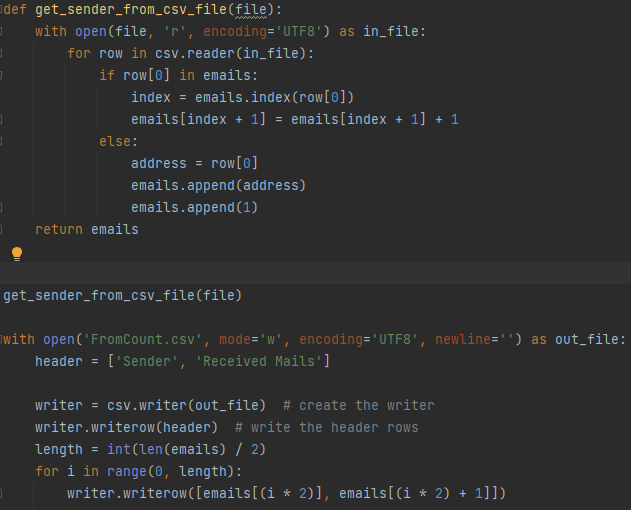
\includegraphics[width=0.75\textwidth]{images/Count_Received_Mails_Count_Sender.PNG}
    \caption{Python Code - Zählen der erhaltenen E-Mails und auflisten nach Absender} 
    \label{fig:countemailssender}
\end{figure}

\begin{figure}
    \centering
    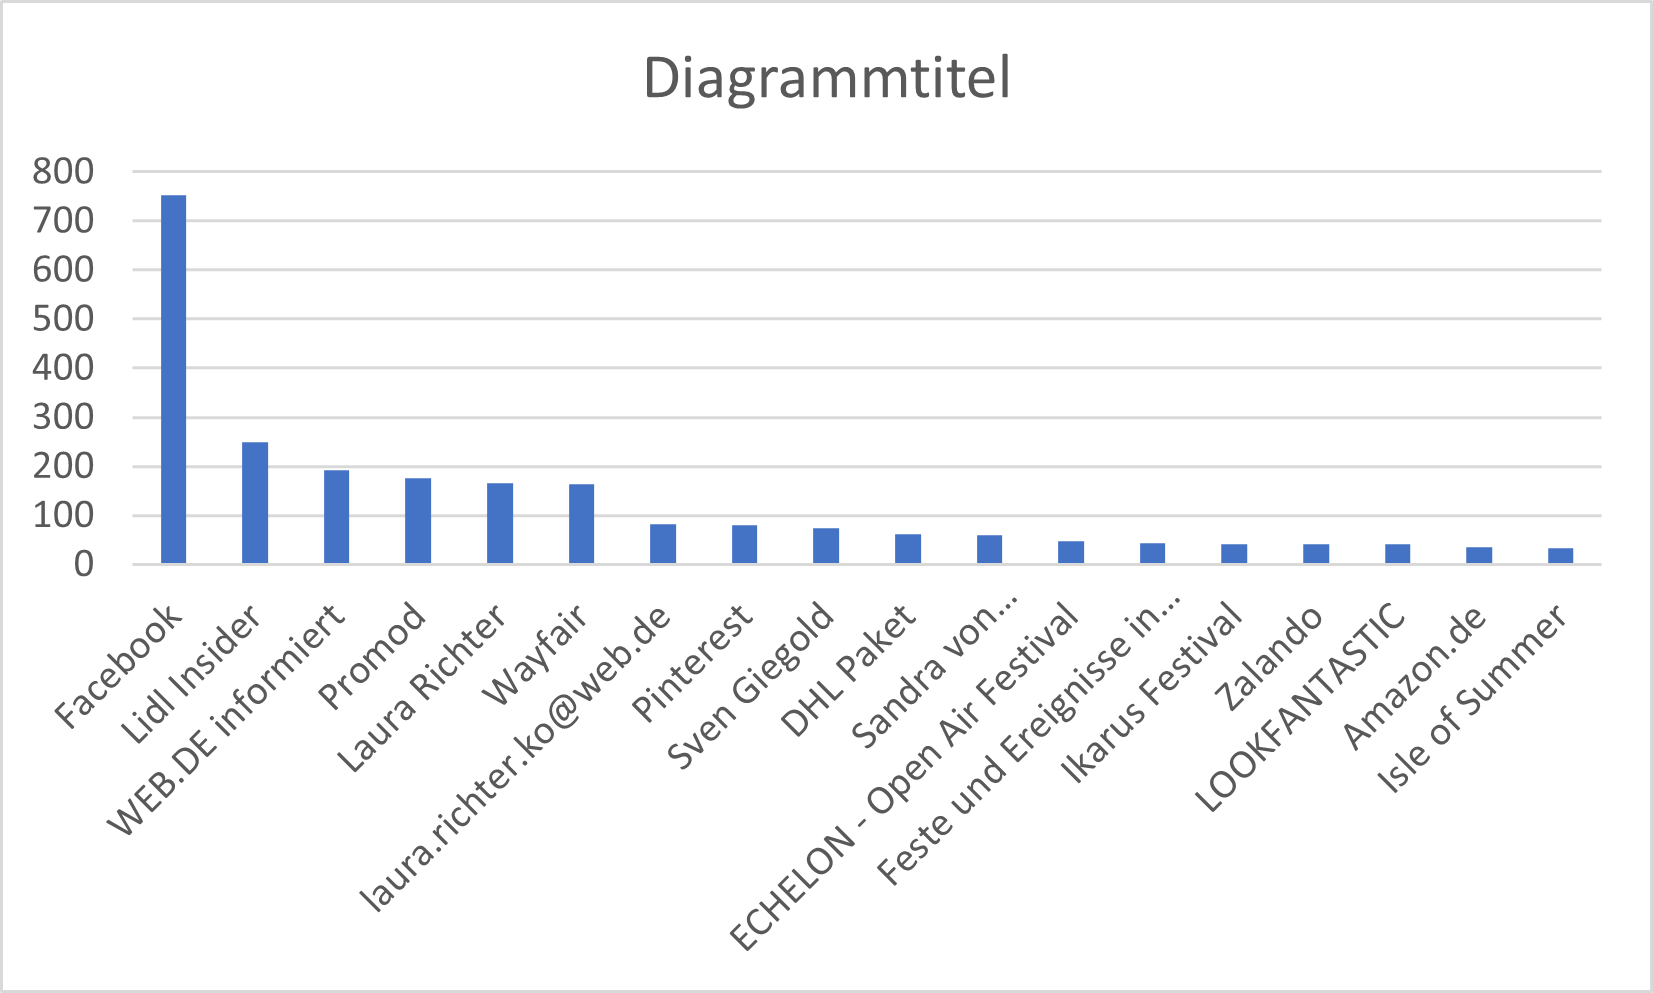
\includegraphics[width=0.75\textwidth]{images/Auswertung_Empfange_Emails.png}
    \caption{Absender mit mehr als 100 gesendeten Mails - Datensatz mit 4102 E-Mails} 
    \label{fig:receivedemails}
\end{figure}

\begin{figure}
    \centering
    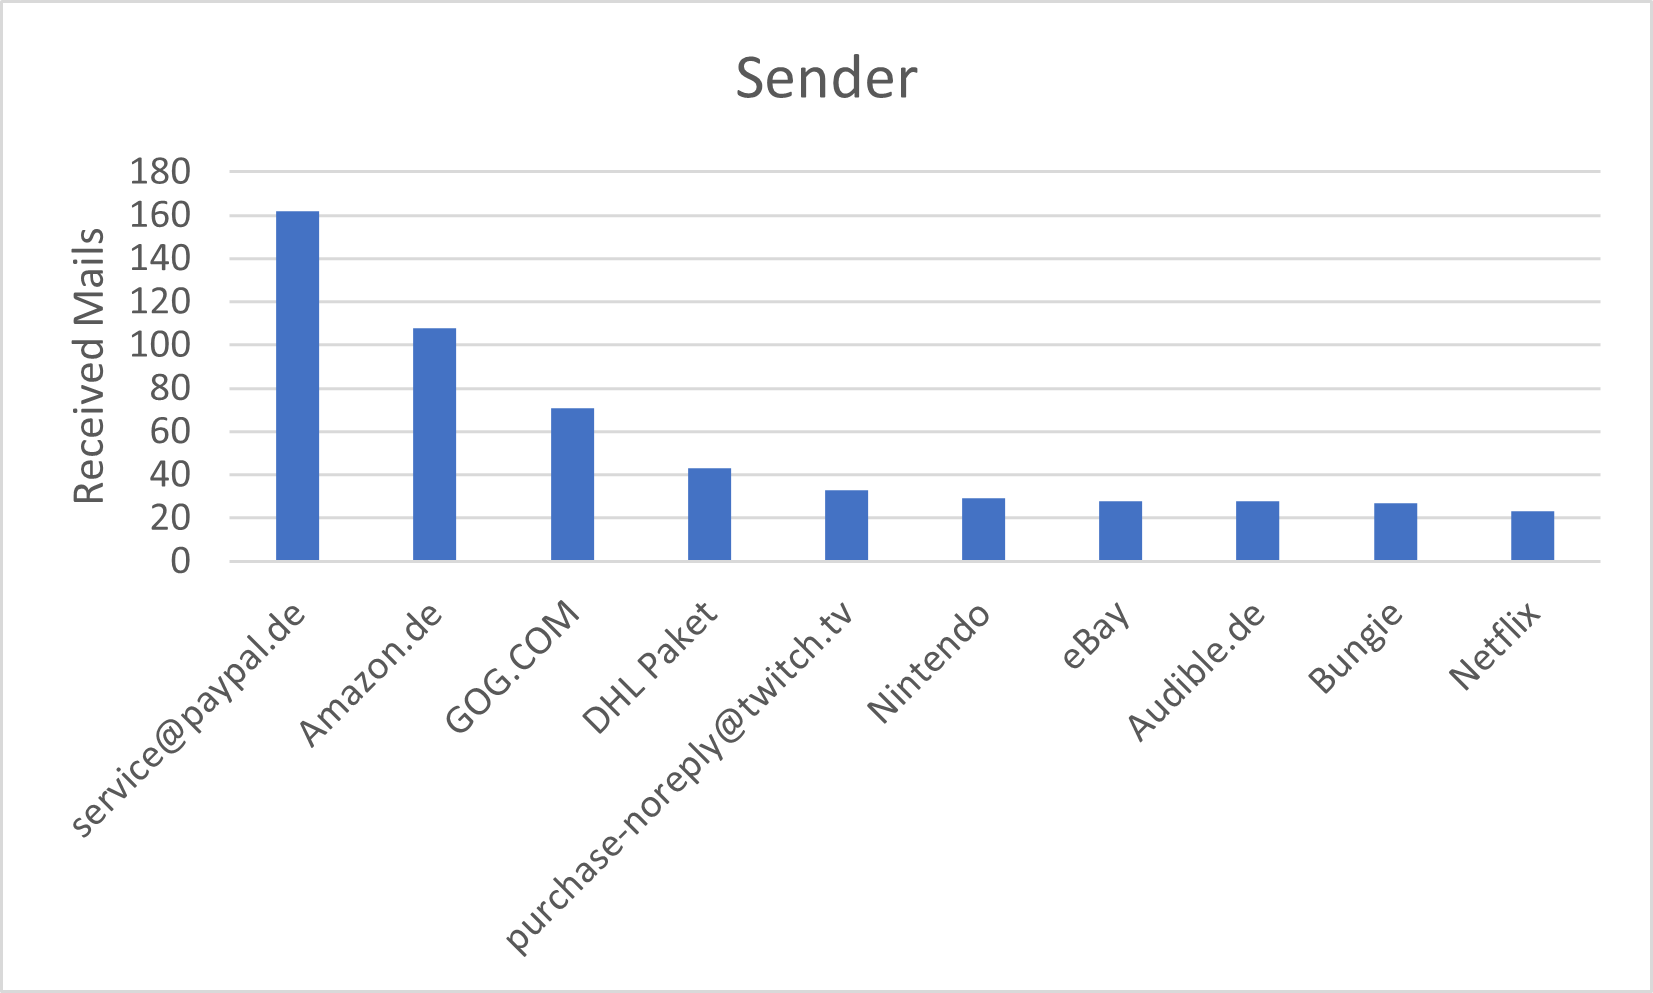
\includegraphics[width=0.75\textwidth]{images/Merged_Auswertung_Empfange_Emails.png}
    \caption{Absender mit mehr als 100 gesendeten Mails - Datensatz mit 6692 E-Mails} 
    \label{fig:receivedemailsmerged}
\end{figure}